\section{Architecture}


\emph{LLAP}, as the name suggests is a long running collection of persistent daemons, which by virtue of being always on side-steps the
overheads of interacting with a large scale resource manager such as YARN\cite{YARN} while executing very short running queries. 

In addition to
that, the long running nature of the processing framework allows for the JDK Hotspot profiling optimizer to collect enough runtime information
to compile the core vectorized loops into \emph{SIMD} native code. To feed this CPU efficient operator pipeline, the data fetching from the storage layer
had to be revamped to buffer into temporary buffer pools so that the operator pipeline is never starved by the vagaries of the networked file
system layer. Since several processing queries share the same data sets, it is incredibly wasteful to discard buffer pools after execution which
naturally led into a cache model which can keep the uncompressed buffers in memory. To reduce the amount of data being fetched for caching, the 
buffers are held as independent columns so that the fetcher can populate a fraction of columns to match the column projections which were involved
during the scan.  The columnar buffers are not unpacked into rows during caching, so the cache maintains all the compression characteristics of the columns such 
as RLE, delta or dictionary encoding. To avoid large GC pauses associated with a large number of indepenent heap objects present in the process heap, 
these cache objects are maintained an off-heap allocator which can be backed by RAM or alternate fast memory mapped storage (NVMe/NVDIMM). The ORC format brings 
additional metadata along  with the columnar layout, which allows for the cache to selectively hold
only the bloom filter indexes or the min-max boundaries for a row-group which was filtered as part of the index miss, eventhough none of the data ever made it
into cache. These two architectural features coincide to provide an incremental additive, but limited cache across queries which follow drill-down and multi-dimension 
access patterns.

LLAP is not a SQL execution engine and neither is it a standardized store for data, but exists as an accelerated access layer with awareness of the relational
model behind the files laid out on disk, dealing with data as column \& row-groups instead of treating it as offsets. LLAP will work within existing, process-based Hive execution to preserve the scalability and versatility of Hive.  It will not replace the existing execution model but enhance it.

To that effect, the architecture of LLAP follows these .

\begin{enumerate}
\item \textbf{Entirely optional.} Hive will continue to work without them and will also be able to bypass them even if they are deployed and operational.  Feature parity with regard to language features will be maintained. 
\item \textbf{Stateless.} Any request to an LLAP node will contain the data location and metadata. It will process local and remote locations; locality will be the caller’s responsibility.
\item \textbf{Recovery/resiliency.} Failure and recovery is simplified because any data node can still be used to process any fragment of the input data. The Tez AM can thus simply rerun failed fragments on the cluster.
\item \textbf{Partial execution.} The result of the work performed by an LLAP daemon can either form part of the result of Hive query, or be passed on to external Hive tasks, depending on the query.
\item \textbf{Communication between nodes.} LLAP nodes will be able to share data (e.g., fetching partitions, broadcasting fragments). This will be realized with the same mechanisms used today in Tez.
\item \textbf{External orchestration engines.} Overall execution will be scheduled and monitored by an existing Hive execution engine such as Tez; transparently over both LLAP nodes, as well as regular containers.  
\item \textbf{Integration with YARN.} LLAP is not external to YARN. LLAP resources are obtained and monitored via YARN. 
\end{enumerate}

\begin{figure*}
\centering
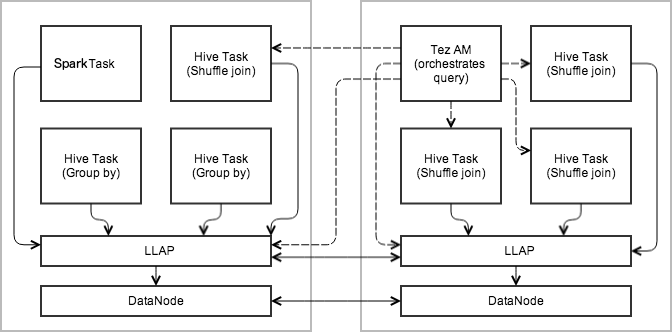
\includegraphics[width=\textwidth]{figures/arch1.png}
\caption{LLAP: as an accelerator}
\label{fig:arch1}
\end{figure*} 

The query engine remains Hive, running Hive
SQL operators while using Tez's DAG execution engine to execute the DAG across failure scenarios and to handle deadlock pre-emption within 
the DAG where multiple vertexes are in motion. This Hybrid execution model highlighted in Figure~\ref{fig:arch1}, in its simplest form 
converts LLAP into a tabular data reader service replacing direct interactions with the networked filesystem. While short running queries
can be run within LLAP entirely, the relational model offered by this interface into data is preferred over the file centric model which
can offer no security beyond file permissions. This change of roles allows for a process boundary between the user code executing within the 
hybrid tasks and allow LLAP to act as gatekeeper for columnar access control, column masking and cell level security.
